\section{Difa Al Fansha}

\subsection{Teori}
	%%Nomor 1
	\subsubsection{Jelaskan dengan ilustrasi gambar sendiri apa perbedaan antara vanilla GAN dan cGAN}
	\hfill\\
	Vanilla GAN memakai data noise yang di proses menjadi data fake sedangkan cGAN memakai latent space atau label untuk generator.
	Generator dan diskriminator adalah perceptron multi-layer sederhana. perceptron merupakan metode JST sederhana menggunakan algoritma training untuk melakukan klasifikasi secara linear.
	Perceptron digunakan untuk melakukan klasifikasi sederhana dan membagi data untuk menentukan data ana yang masuk dalam klasifikasi dan data mana yang diluar klasifikasi.
	Vanilla GAN mengoptimalkan persamaan mtk menggunakan keturunan gradien stokastik.
	
	\begin{figure}[H]
		\begin{center}
		 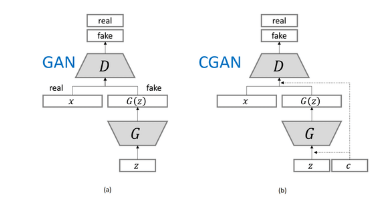
\includegraphics[width=10cm]{figures/1174076/figures9/teori1.png}
		 \caption{}	
		\end{center}
	\end{figure}

	%%Nomor 2
	\subsubsection{Jelaskan dengan ilustrasi gambar sendiri arsitektur dari Age-cGAN}
	\hfill\\
	AgecGan terdiri dari empat jaringan: Encoder, FaceNet, Jaringan Generator, dan jaringan diskriminator. 
	Encoder, kita belajar pemetaan invers gambar wajah masukan dan kondisi usia dengan vektor laten. 
	FaceNet adalah jaringan pengenalan wajah yang mempelajari perbedaan antara gambar input x dan gambar yang direkonstruksi. 
	Kami memiliki jaringan Generator, yang mengambil representasi tersembunyi yang terdiri dari gambar wajah dan vektor kondisi dan menghasilkan gambar. 
	Jaringan diskriminator adalah untuk mendiskriminasikan antara gambar nyata dan gambar palsu. 
	Masalah dengan cGANs adalah bahwa mereka tidak dapat mempelajari tugas pemetaan terbalik masukan gambar x dengan atribut y ke vektor laten z. 
	Solusi untuk masalah ini adalah dengan menggunakan jaringan Encoder. 
	Kita dapat melatih jaringan encoder untuk memperkirakan pemetaan terbalik dari input Images x	
	
	%%Nomor 3
	\subsubsection{Jelaskan dengan ilustrasi gambar sendiri arsitektur encoder network dari AgecGAN}
	\hfill\\
	Arsitektur encoder biasanya digunakan untuk memodelkan struktur manifold dan membalikkan encoder untuk memproses data.

	\begin{figure}[H]
		\begin{center}
		 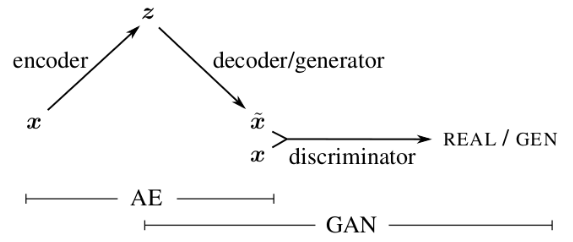
\includegraphics[width=10cm]{figures/1174076/figures9/teori3.png}
		 \caption{}	
		\end{center}
	\end{figure}
	
	%%Nomor 4
	\subsubsection{Jelaskan dengan ilustrasi gambar sendiri arsitektur generator network dari AgecGAN}
	\hfill\\
	Encoder mempelajari pemetaan terbalik dari gambar wajah input dan kondisi usia dengan vektor laten Z. Jaringan encoder menghasilkan vektor laten dari gambar input. Jaringan Encoder adalah CNN yang mengambil gambar dari dimensi (64, 64, 3) dan mengubahnya menjadi vektor 100 dimensi. Ada empat blok konvolusional dan dua lapisan padat. Setiap blok konvolusional memiliki lapisan konvolusional, diikuti oleh lapisan normalisasi batch, dan fungsi aktivasi kecuali lapisan konvolusional pertama.
	
	\begin{figure}[H]
		\begin{center}
		 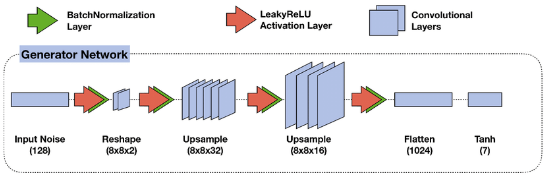
\includegraphics[width=10cm]{figures/1174076/figures9/teori4.png}
		 \caption{}	
		\end{center}
	\end{figure}
	
	%%Nomor 5
	\subsubsection{Jelaskan dengan ilustrasi gambar sendiri arsitektur discriminator network dari Age-cGAN} 
	\hfill
	Arsitektur diskriminator adalah CNN yang dapat menerima input gambar yang berukuran 28,28 serta menghasilkan angka biner yang menyatakan apakah data yang diinputkan merupakan dataset asli atau gambar dataset palsu.
	
	\begin{figure}[H]
		\begin{center}
		 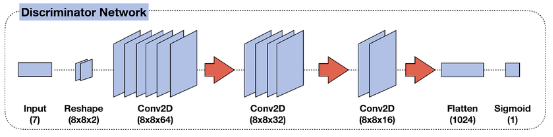
\includegraphics[width=10cm]{figures/1174076/figures9/teori5.png}
		 \caption{}	
		\end{center}
	\end{figure}
	
	%%Nomor 6
	\subsubsection{Jelaskan dengan ilustrasi gambar apa itu pretrained Inception-ResNet-2 Model}
	\hfill\\
	Pre-Trained Network atau Transfer Learning merupakan suatu metode penyelesaian yang memanfaatkan model yang sudah dilatih terhadap suatu dataset untuk menyelesaikan masalah dengan cara menggunakan sebagai starting point, memodifikasi dan mengupdate parameternya, sehingga sesuai dengan dataset yang baru.
	Inception resNet 2 adalah jaringan saran konvolusional yang dilatih lebih dari satu juta gambar
	
	\begin{figure}[H]
		\begin{center}
		 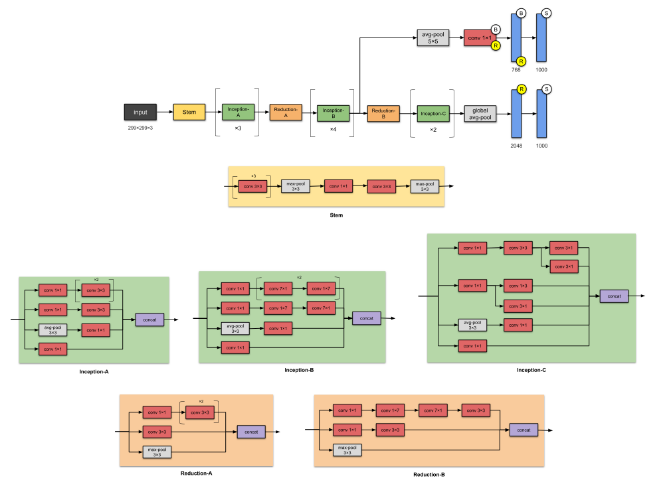
\includegraphics[width=10cm]{figures/1174076/figures9/teori6.png}
		 \caption{}	
		\end{center}
	\end{figure}
	
	%%Nomor 7
	\subsubsection{Jelaskan dengan ilustrasi gambar sendiri arsitektur Face recognition network Age-cGAN}
	\hfill\\
	Face Recognition merupakan salah satu sistem yang mengimplementasi Deep Learning yang dapat mengenali wajah secara fisik dari gambar digital atau video frame.
	
	\begin{figure}[H]
		\begin{center}
		 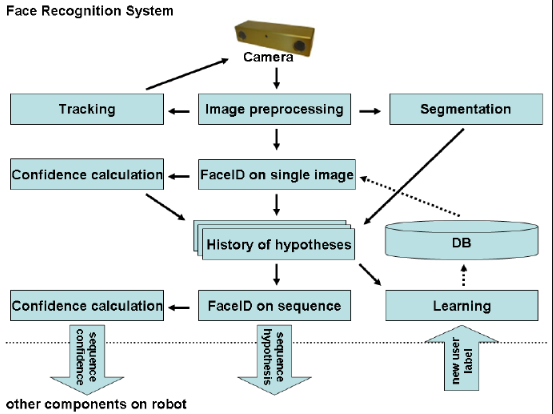
\includegraphics[width=10cm]{figures/1174076/figures9/teori7.png}
		 \caption{}	
		\end{center}
	\end{figure}
	
	%%Nomor 8
	\subsubsection{Sebutkan dan jelaskan serta di sertai contoh-contoh tahapan dari Age-cGAN}
	\hfill\\
	Terdapat 3 tahapan : 
	\begin{itemize}
		\item Conditional GAN, Melatih generator dan discriminator.
		\item Initial Lantent Vector Approxmation, Melatih encoder.
		\item Latent vector optimization, Mengoptimalkan encode dan generator
	\end{itemize}

	%%Nomor 9
	\subsubsection{Berikan contoh perhitungan fungsi training objektif}
	\hfill\\
	Objektif Trainning ialah untuk meminimalkan loss function sebagai log likelihood function yang diberikan pada persamaan dimana D melambangkan trainning data.
	
	%%Nomor 10
	\subsubsection{Berikan contoh dengan ilustrasi penjelasan dari Initial latent vector approximation}
	\hfill\\
	Latent vector approximation kemampuan untuk membuat gamar yang realistis dan tajam serta menghasilkan gambar wajah pada usia target.
	
	\begin{figure}[H]
		\begin{center}
		 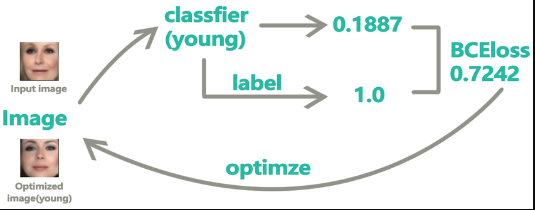
\includegraphics[width=10cm]{figures/1174076/figures9/teori10.png}
		 \caption{}	
		\end{center}
	\end{figure}

	%%Nomor 11
	\subsubsection{Berikan contoh perhitungan latent vector optimization}
	\hfill\\
	Perhitungan lantent optimization menggunakan metode yang relatif sederhana, tergantung pada jumlah kecil parameter yang diperlukan, sehingga pada latent optimization dapat memetakan setiap gambar x dari dataset ke vektor acak dimensi rendah zi dalam ruang laten z.
	
	\begin{figure}[H]
		\begin{center}
		 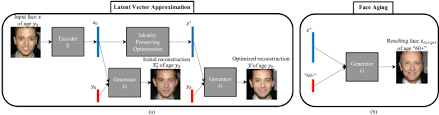
\includegraphics[width=10cm]{figures/1174076/figures9/teori11.png}
		 \caption{}	
		\end{center}
	\end{figure}
	
\subsection{Praktek}
 
	%%Nomor 1
	\subsubsection{Jelaskan bagaimana cara ekstrak file dataset Age-cGAN menggunakan google colab}
	\hfill\\
		\lstinputlisting[firstline=1, lastline=4]{src/1174076/src9/1174076.py}


	%%Nomor 2
	\subsubsection{Jelaskan bagaimana kode program bekerja untuk melakukan load terhadap dataset yang sudah di ekstrak, termasuk bagaimana penjelasan kode program perhitungan usia}
	\hfill\\

		\lstinputlisting[firstline=6, lastline=31]{src/1174076/src9/1174076.py}


	%%Nomor 3
	\subsubsection{Jelaskan bagaimana kode program The Encoder Network bekerja dijelaskan dengan bahawa awam dengan ilustrasi sederhana}
	\hfill\\
	Proses Encoder berfungsi untuk mempelajari pemetaan terbalik dari gambar wajah dan kondisi usia dengan vector latent Z.

			\lstinputlisting[firstline=33, lastline=73]{src/1174076/src9/1174076.py}

	
	%%Nomor 4
	\subsubsection{Jelaskan bagaimana kode program The Generator Network bekerja dijelaskan dengan bahawa awam dengan ilustrasi sederhana}
	\hfill\\
	Proses Generator agar bekerja dengan baik dibutuhkan representasi dari gambar wajah dan vector kondisi sebagai inputan yang menghasilkan sebuah gambar.

		\lstinputlisting[firstline=75, lastline=104]{src/1174076/src9/1174076.py}


	%%Nomor 5
	\subsubsection{Jelaskan bagaimana kode program The Discriminator Network bekerja dijelaskan dengan bahawa awam dengan ilustrasi sederhana}
	\hfill\\
	Proses Discriminator untuk membedakan antara gambar asli dan gambar palsu.

		\lstinputlisting[firstline=116, lastline=148]{src/1174076/src9/1174076.py}
	
	
	%%Nomor 6
	\subsubsection{Jelaskan bagaimana kode program Training cGAN bekerja dijelaskan dengan bahawa awam dengan ilustrasi sederhana}
	\hfill\\
	Proses Training cGAN ini dengan load file .mat pada dataset lalu epoch sebanuak 500 kali.

		\lstinputlisting[firstline=150, lastline=167]{src/1174076/src9/1174076.py}

	
	%%Nomor 7
	\subsubsection{Jelaskan bagaimana kode program Initial dan latent vector approximation bekerja dijelaskan dengan bahawa awam dengan ilustrasi sederhana}
	\hfill\\
	
		\lstinputlisting[firstline=169, lastline=217]{src/1174076/src9/1174076.py}
	Initial dan Latent Vector Approximation bekerja melakukan predicsi epoch yang telah di buat sebanyak 500 kali, dan nanti hasilnya ada di folder result.


\subsection{Penangan Error}
	
	\subsubsection{Screenshoots Error}\hfill\\
	
	\subsubsection{Tuliskan kode eror dan jenis errornya}\hfill\\
	 
	\subsubsection{Solusi pemecahan masalah error tersebut}\hfill\\
	
\subsection{Bukti Tidak Plagiat}
\hfill\\
	\begin{figure}[H]
		\centerline{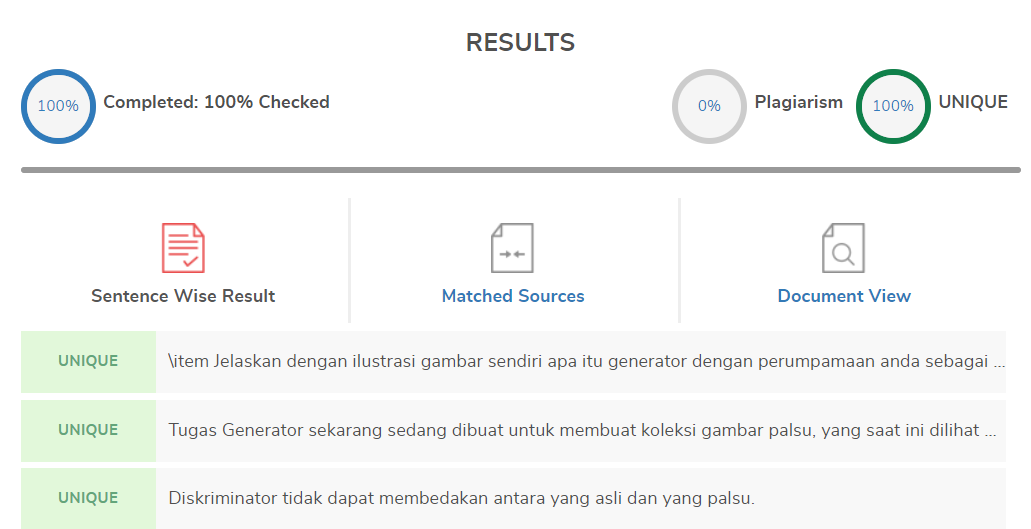
\includegraphics[width=10cm]{figures/1174076/figures9/plagiat.png}}
		\caption{Bukti Tidak Plagiat}
		\label{labelgambar}
	\end{figure}

\subsection{Link Youtube:}
https://www.youtube.com/watch?v=RYcrSdyEaQc
	